Intermolecular interactions dictate thermodynamic properties of molecular solids, layered materials, and soft matter in general, including most biological matter, and govern molecular adsorption and self-assembly, which includes most biological processes.
Van der Waals (vdW) forces, which emerge from correlations in the quantum fluctuations of electron density, are the only kind of intermolecular interactions with quantum-mechanical origin, and consequently give rise to a wide spectrum of physical phenomena, ranging from attraction between small organic molecules~\citep{LondonZP30}, to shifts of optical spectra in nanoparticles~\citep{LuoP14}, to the macroscopic Casimir effect~\citep{JaffePRD05}.
As a result, vdW interactions have been, and are increasingly so, one of the prime targets of material modeling, which has led to a plethora of approaches that either treat vdW forces implicitly or model them explicitly~\citep{KlimesJCP12,HermannCR17}.
These include quantum Monte--Carlo~\citep{AmbrosettiJPCL14}, coupled clusters~\citep{YangS14}, random-phase approximation~\citep{LuPRL09}, nonlocal density functionals~\citep{DionPRL04,VydrovPRL09}, and coarse-grained approaches, which range from pairwise~\citep{GrimmeJCC04,BeckeJCP07,TkatchenkoPRL09} to many-body models~\citep{TkatchenkoPRL12,SilvestrelliJCP13}.
From theoretical perspective, this status quo is undesirable, because different models often give disparate pictures of the nature of vdW forces, which leads to incoherent understanding of vdW interactions in molecules and materials.
From practical perspective, the three main characteristics of a method are its applicability, accuracy, and computational efficiency, and so far, no single method has satisfied all three requirements with respect to vdW forces to such a degree, that it would be reliably applicable to a broad range of realistic materials.

In this Letter, we present a unified density-functional model of vdW interactions that combines ingredients from nonlocal functionals and coarse-grained models, inheriting broad applicability of the former and good accuracy of the latter, while retaining the computational efficiency of both.
We use the polarizability functional of \citet{VydrovPRA10} (VV), the Hamiltonian form of the many-body dispersion (MBD) model~\citep{TkatchenkoJCP13}, the idea of normalization to jellium via a zero-gradient limit from the VV10 nonlocal functional~\citep{VydrovJCP10a}, and normalization to reference free-atom vdW parameters coined by the exchange-hole dipole moment model~\citep{BeckeJCP06} and the vdW model of \citet{TkatchenkoPRL09} (TS).
Compared to the range-separated self-consistently screened (rsSCS) variant of MBD~\citep{AmbrosettiJCP14}, the use of the VV polarizability functional in the new model enables consistent treatment of ionic compounds, and normalization to jellium enables effective modeling of adsorption on metallic surfaces comparable to the surface variant of the TS model~\cite{RuizPRL12}, while normalization to free-atom reference values restores the accuracy of the VV polarizability functional for transition metals.
Furthermore, the VV polarizability functional---unlike approaches based on atomic volume---
is able to capture short-range many-body polarization effects, so that the short-range screening of atomic polarizabilities is not needed in the new model, reducing the overall computational cost by an order of magnitude compared to MBD@rsSCS\@.
We demonstrate on a series of benchmark calculations that our new model enables for the first time consistent treatment of vdW interactions in covalent, ionic, and hybrid metal-organic interfaces by a single method, while achieving the accuracy of the best approaches for each individual class of systems.

The central proposition of the new model, dubbed MBD@VV, is to parameterize the Hamiltonian of the MBD model with the VV polarizability functional.
The MBD Hamiltonian describes a system of charges in harmonic potentials---Drude oscillators---characterized by their static polarizabilities $\alpha_{0,i}$ and resonance frequencies $\omega_i$, and interacting via a long-range dipole potential $\mathbf T^\mathrm{lr}(\mathbf R)\equiv f(R)\mathbf T(\mathbf R)$,
\begin{multline}
  H^\text{MBD}(\{\alpha_{0,i},\omega_i\})=\sum_i-\frac12\nabla_{\xi_i}^2+\sum_i\frac12\omega_i^2\xi_i^2 \\
  +\frac12\sum_{ij}\omega_i\omega_j\sqrt{\alpha_{0,i}\alpha_{0,j}}\boldsymbol{\xi}_i\cdot\mathbf T^\mathrm{lr}_{ij}\boldsymbol{\xi}_j
\end{multline}
where $\boldsymbol\xi_i\equiv\sqrt{m_i}\mathbf x_i$ are mass-weighted displacements of the charges.
To calculate the vdW energy, each oscillator is parametrized such that it models the polarization response of a single atom in a molecule or material.
The interaction energy of this model system---the vdW energy---is then readily obtained by direct diagonalization of the Hamiltonian.
The shortcomings of MBD@rsSCS in description of ionic compounds and hybrid interfaces do not originate in the form of the Hamiltonian, but rather in the parametrization of the oscillators via Hirshfeld volumes.

In MBD@VV, we parametrize the oscillators by coarse-graining the VV polarizability density to Hirshfeld fragments~\citep{HirshfeldTCA77,SatoJCP09,SatoJCP10}.
The VV functional is a semilocal functional of the electron density $n(\mathbf r)$, which models local isotropic dynamic polarizability density $\alpha(\mathbf r,\mathrm iu)$,
\begin{equation}
   \alpha^\text{VV}[n](\mathrm iu)=\frac{n}{\frac{4\pi}3n+C\frac{|\boldsymbol\nabla n|^4}{n^4}+u^2}
   \label{eq:vv-functional}
\end{equation}
where $\mathrm iu$ is imaginary frequency and $C$ is an empirical parameter fitted to reproduce a reference set of $C_6$ coefficients.
The atomic dynamic polarizabilities are obtained by integrating the polarizability density with Hirshfeld weights $w_i^\text{H}(\mathbf r)$,
\begin{equation}
  \alpha_i^\text{VV}(\mathrm iu)=\int\mathrm d\mathbf r\,w_i^\text{H}(\mathbf r)\alpha^\text{VV}[n](\mathbf r,\mathrm iu)
\end{equation}
The effective oscillator frequencies are calculated such as to reproduce the same $C_6$ coefficients for the oscillators as if calculated directly from $\alpha_i(\mathrm iu)$ via the Casimir--Polder formula,
\begin{equation}
  \omega_i^\text{VV}=\frac43\frac{C_{6,i}^\text{VV}}{\alpha_i^\text{VV}{(0)}^2},\quad
  C_{6,i}^\text{VV}=\frac3\pi\int_0^\infty\mathrm du\,\alpha_i^\text{VV}{(\mathrm iu)}^2
\end{equation}
Unlike in approaches that use Hirshfeld fragments to define atomic volumes, the particular choice of the atomic partitioning in MBD@VV is mostly inconsequential, because it only influences local redistribution of the polarizability between atoms---not total polarizability, nor polarizability distribution over larger length scales.

Already this plain combination of the MBD model and VV polarizability functional gives a substantial improvement in description of ionic systems over MBD@rsSCS, thanks to the versatility of the VV functional.
But when combined with semilocal density-functional theory (DFT), it still suffers from double-counting of electron correlation in metallic systems (slowly-varying electron density regions), and lacks in accuracy for organic compounds with respect to state-of-the-art vdW models.
To solve these two issues, we borrow two techniques from the VV10 nonlocal functional and the TS model.
First, we normalize MBD@VV such that it gives zero vdW energy for jellium by subtracting the portion of the polarizability that comes from metallic electron density regions.
Second, we normalize the atomic VV polarizabilities and $C_6$ coefficients to reproduce the respective exact quantities for free atoms.

Most exchange--correlation (XC) functionals are exact for jellium by construction, even though the portion of electron correlation coming from plasmons is long-ranged and should not in principle be accounted for by semilocal XC functionals.
As a result of this construction, most XC functionals describe accurately the electron correlation \emph{within} slowly-varying density regions, such as those found in metals, and no correction for vdW forces is needed.
This is unlike in all other cases, where semilocal functionals neglect long-range vdW interactions.
Furthermore, the interactions \emph{between} such regions and other regions of the electron density are effectively screened by the conducting electrons.
At the same time, these metallic-density regions contribute dominantly to the polarizability in the VV functional (in principle the local polarizability of a conductor should be infinite) and hence to the vdW energy in any vdW model, in which the VV functional would be used directly.
When combined with semilocal DFT, this would result in overpolarization and overbinding of bulk metals as well as of adsorbates on metallic surfaces.
To avoid this double-counting of the long-range electron correlation, the VV10 nonlocal functional subtracts the limit of itself as the density gradient approaches zero from the final VV10 vdW energy expression, such that the vdW energy is equal to zero for jellium,
\begin{equation}
  E_\text{vdW}^\text{VV10} = E^\text{VV10}[n]-\big(E^\text{VV10}\big|_{\boldsymbol\nabla n\rightarrow0}\big)[n]
\end{equation}
Such an approach cannot be used directly in a many-body model such as MBD, so we devised a related construction.

\begin{figure}[t!]
\begin{tikzpicture}
\node[below right] at (0,0) {\bfseries a};
\node[below right, inner sep=0pt] at (0,0) {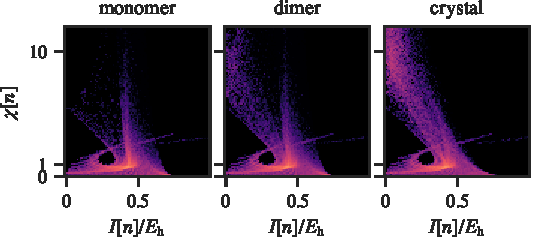
\includegraphics{../media/benzene.pdf}};
\node[below right] at (0,-4.3) {\bfseries b};
\node[below right, inner sep=0pt] at (0,-4.3) {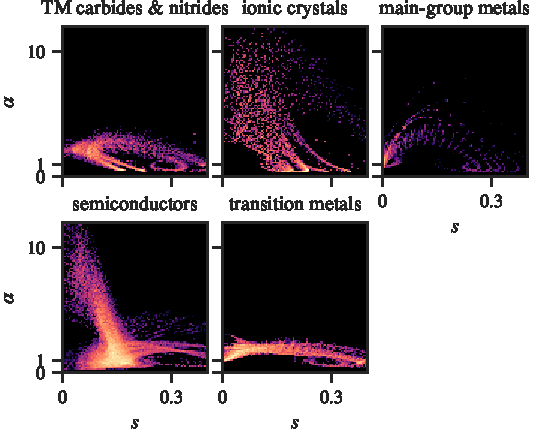
\includegraphics{../media/solids-hists.pdf}};
\end{tikzpicture}
\caption{\textbf{Polarizability distributions of reduced gradient $s$ and iso-orbital indicator $\chi$.}
Precisely, the plotted distributions are $\alpha^\text{VV}(s',\chi')=\int\mathrm d\mathbf r\delta(s(\mathbf r)-s')\delta(\chi(\mathbf r)-\chi')\alpha^\text{VV}(\mathbf r)$ such that the total polarizability is equal to $\iint\mathrm ds\mathrm d\chi\,\alpha^\text{VV}(s,\chi)$.
(\textbf a) Benzene monomer, dimer, and crystal.
Each distribution is normalized to one benzene molecule.
(\textbf b) 63 simple solids divided to five groups (see SI for details).
Each distribution is normalized to 62 (a.\,u.), the VV polarizability of a benzene monomer, to share a single color scale with \textbf{a}.
}\label{fig:pol-hists}
\end{figure}

Rather than evaluating the interaction of the metallic-density regions and than subtracting it, as in VV10, we do not evaluate it in the first place by smoothly cutting of the contribution of these regions to the polarizability.
These regions can be distinguished using the combination of two local dimensionless electron-density descriptors: the reduced gradient $s$ and the iso-orbital indicator $\chi$~\citep{BeckeJCP90,KummelMP03,SunPRL13},
\begin{equation}
  s[n]=\frac{|\boldsymbol\nabla n|}{2{(3\pi^2)}^\frac13n^\frac43},\qquad
  \chi[n]=\frac{\tau^\text{KS}[n]-\tau^\text{W}[n]}{\tau^\text{unif}[n]}
\end{equation}
where $\tau[n]=\sum_i|\boldsymbol\nabla\phi_i|^2/2$ is the positive kinetic energy density of occupied orbitals $\phi_i$, which for single-orbital densities reduces to the von Weizsäcker kinetic energy density, $\tau^\text W[n]=|\boldsymbol\nabla n|^2/8n$, and for jellium to $\tau^\mathrm{unif}[n]=3(3\pi^2)^{2/3}n^{5/3}/10$.  % chktex 3
The density gradient alone is not sufficient to characterize metallic density.
In particular, both $s\sim0$ and $\chi\sim1$ must be true for density to be metallic, whereas $s\sim0$ and $\chi\sim0$ corresponds to centers of covalent bonds (dominated by a single bonding orbital) and $s\sim0$ and $\chi\gg1$ signifies overlaps of electron density tails that occur between noncovalently bound systems.
Since the normalization of VV10 to jellium uses only the density gradient, it partially omits also contributions from covalent bonds and density-tail overlaps.
By using the iso-orbital indicator, we can make MBD@VV more precise.

Figure 3 presents polarizability distributions of $s$ and $\chi$ in benzene compounds and in a set of simple solids, and shows that they are very sensitive to the nature of the bonding in a molecular or material.
In a organic molecule such as benzene (Figure~\ref{fig:pol-hists}a), the vast majority of the polarizability
comes from electron density with $s>0.1$ while the small remainder comes
from low-gradient regions with $\chi<1$.
With the introduction of intermolecular interactions in a benzene dimer and crystal, a significant amount of polarizability comes from regions with $\chi\gg1$, despite the electron density being low in such regions.
A richer spectrum of patterns can be found in simple solids (Figure~\ref{fig:pol-hists}b).
Most similar to the benzene compounds is the group of semiconductors.
In contrast, the vast majority of the polarizability in main-group metals comes from jellium-like regions near $(s,\chi)=(0,1)$, as expected.
In transition metals, the polarizability is distributed over a wider range of the reduced gradient along the $1<\chi<2$ strip, with larger part still coming from low-gradient regions.
These features are largely shared by the transition-metal carbides and nitrides, but notably the near neighborhood of $(s,\chi)=(0,1)$ does not contribute.
In simple ionic solids, which do not feature covalent bonds, most of the
polarizability comes from single-orbital regions ($\chi<1$), although a
significant amount also comes from noncovalent orbital-overlap regions.

Based on these numerical results, we devise a smooth cutoff function $0\leq g(s,\chi)\leq 1$ of the two density descriptors that distinguishes the nonmetallic density regions, and define the nonmetallic portion of polarizability density as
\begin{equation}
  \alpha^\mathrm{VV'}[n]=g(s,\chi)\alpha^\text{VV}[n]
\end{equation}
The exact shape of the cutoff function is to a certain degree arbitrary (the analytical form is presented in the SI), but thanks to the unambiguous distinction in the polarizability distributions between organic compounds and metals, the results are not too sensitive to a particular choice.
In general terms, it can be characterized as being zero in the largest possible region around $(s,\chi)=(0,1)$ without affecting the polarizabilities of organic compounds.
This way, the effective polarizability of a simple metal such as lithium is close to zero in our model, as is the vdW energy, whereas the difference between VV$'$ and VV polarizabilities is less than 2\% on average for organic molecules (the S66 set).

\begin{figure}[t!]
\centering
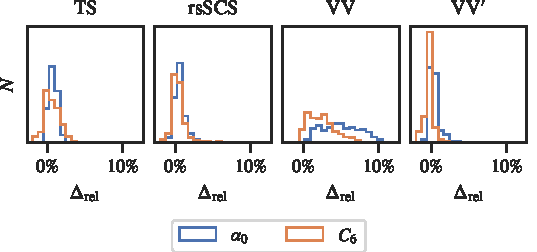
\includegraphics{../media/pol-shifts.pdf}
\caption{\textbf{Distributions of relative changes in atomic polarizabilities and $C_6$ coefficients from monomers to dimers.}
The distributions are calculated over all atoms from all complexes in the S66 data set.
}\label{fig:pol-shifts}
\end{figure}

Apart from proper treatment of metals, we use the cutoff function $g$ for another purpose.
When molecules are brought together to form vdW-bound compounds, the introduction of density-tail overlaps significantly increases the polarizability in a model such as the VV functional (Figure~\ref{fig:pol-hists}a).
For instance, the VV polarizability per molecule goes from 62 (a.\,u.) in benzene monomer, to 67 in benzene dimer, to 92 in benzene crystal.
This effect is an artifact of the VV functional that overbinds increasingly large vdW-bound systems.
To eliminate this issue, we extend the region in which the cutoff function $g$ is zero to all low-gradient regions with $\chi>1$.
This does not affect the polarizabilities of organic monomers, but ensures that the increase in polarizability from monomers to dimers is less than 1\% on average (Figure~\ref{fig:pol-shifts}).

\begin{figure}[t!]
\centering
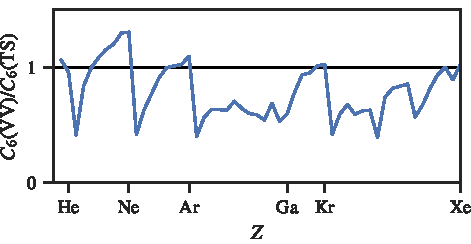
\includegraphics{../media/vv-periodic-table.pdf}
\caption{\textbf{Relative errors in VV polarizabilities of free atoms for first 54 elements.}
}\label{fig:vv-periodic-table}
\end{figure}

The VV polarizability functional is only approximate, which is manifest already for free-atom polarizabilities and $C_6$ coefficients, where accurate reference values are known.
To mitigate this error, we normalize the VV quantities with the ratio of the free-atom polarizabilities and $C_6$ coefficients as calculated by the VV functional and as given by reference calculations,
\begin{equation}
  \alpha_{0,i}^\text{rVV}=\alpha_{0,i}^\text{nmVV}\frac{\alpha_{0,i}^\text{ref,free}}{\alpha_{0,i}^\text{VV,free}},\quad
  C_{6,i}^\text{rVV}=C_{6,i}^\text{nmVV}\frac{C_{6,i}^\text{ref,free}}{C_{6,i}^\text{VV,free}}
\end{equation}
This correction assumes that any error in $\alpha^\text{VV}[n]$ (or $\alpha^\text{nmVV}[n]$) is at least partially transferable from free atoms to atoms in molecules and materials.
Alternatively, this step can be seen as a modification of the TS method \citep{TkatchenkoPRL09}, in which the scaling of reference free-atom quantities by Hirshfeld volumes is replaced with that by VV-derived polarizabilities and $C_6$ coefficients.

Finally, we use the same definition of $\mathbf T^\text{lr}$ as in the MBD@rsSCS variant \citep{AmbrosettiJCP14},
\begin{equation}
  \mathbf T_{ij}^\text{lr}=\frac1{1+\exp\left(-6\Big(\frac{|\mathbf r|}{\beta(R_i^\text{vdw}+R_j^\text{vdw})}-1\Big)\!\!\right)}\boldsymbol\nabla\otimes\boldsymbol\nabla\frac1{|\mathbf r|}\Bigg|_{\mathbf r=\mathbf R_j-\mathbf R_i}
\end{equation}
with the vdW radii $R_i^\text{vdW}$ obtained by scaling free-atom radii with ratio of Hirshfeld volumes in the molecule or material and in free atoms,
\begin{equation}
  R_i^\text{vdW}=R_i^\text{vdW,free}{\left(\frac{V_i^\text{H}}{V_i^\text{H,free}}\right)}^\frac13,\quad
  R_i^\text{vdW,free}=\tfrac52{(\alpha_{0,i}^\text{free})}^\frac17
\end{equation}
The only novel minor modification is that the free-atom radii are calculated from free-atom static polarizabilities \citep{FedorovPRL18} rather than taken as external input.

\section{Results}

\section{Discussion}

Hirshfeld partitioning/Hirshfeld volumes, sensitivity to choice of partitioning.

How double-counting is treated

Discuss short/long-range nature of fluctuations in metals, screening.

Discuss $g_\text{nm}$.

\section{Conclusions}
